\cmfnewsection{Aplicação: Análise de Estabilidade de Redes Baseadas em MMC}{./logos/fundo_tese}{0.15}



%%%%%%%%%%%%%%%%%%%%%%%%%%%%%%%%%%%%%%%%%%%%%%%%%%%%%%%
%%%%%%%%%%%%%%%%%%%%%%%%%%%%%%%%%%%%%%%%%%%%%%%%%%%%%%%
%%%%%%%%%%%%%%%%%%%%%%%%%%%%%%%%%%%%%%%%%%%%%%%%%%%%%%%
\begin{frame}{Estabilidade de Sistemas Baseados em MMC}

\centering
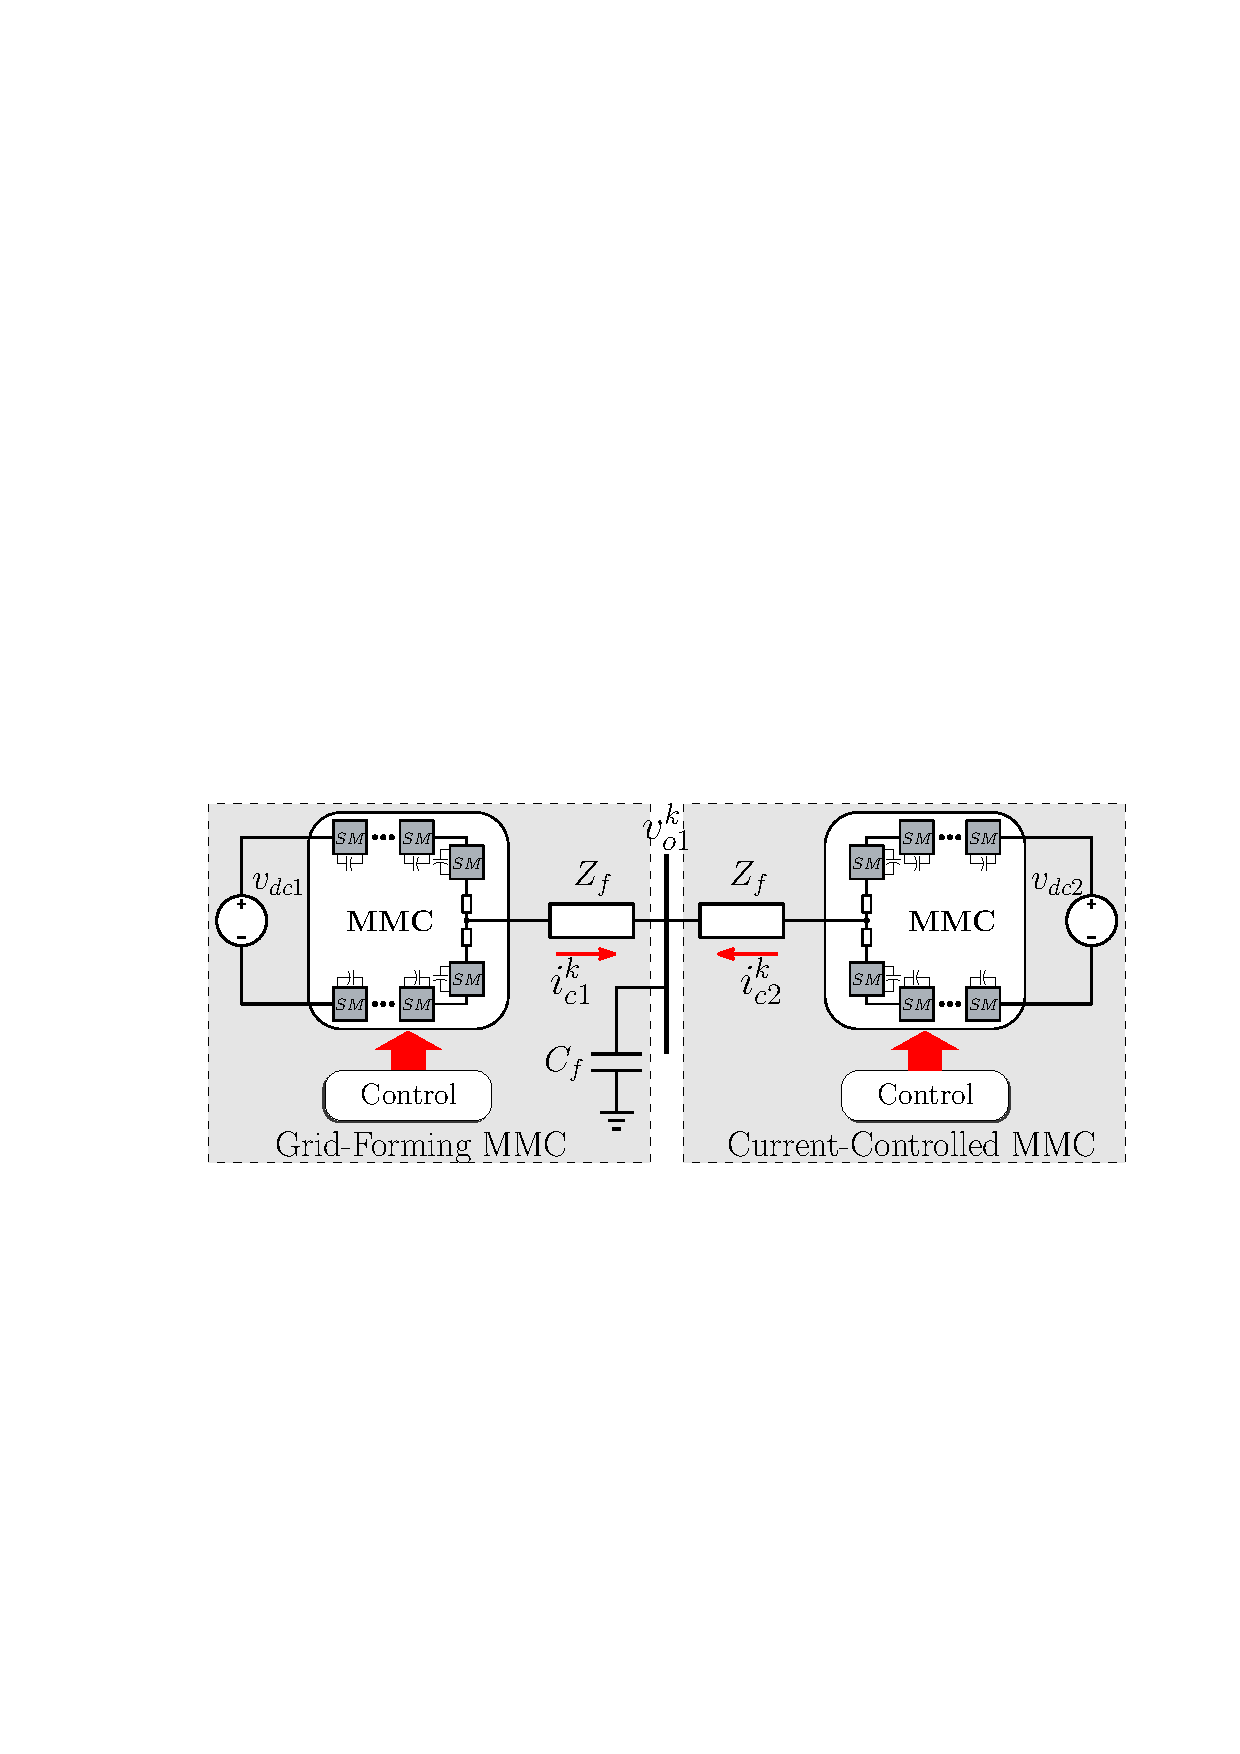
\includegraphics[width=0.9\linewidth]{./figuras/aplicacao/conjunto_MMC5}\\


Por ex.: Inversora de um HVDC
~~~~~~~~~~~~~~
Por ex.: Parque Eólico

\end{frame}



%%
%%%%%%%%%%%%%%%%%%%%%%%%%%%%%%%%%%%%%%%%%%%%%%%%%%%%%%%%
%%%%%%%%%%%%%%%%%%%%%%%%%%%%%%%%%%%%%%%%%%%%%%%%%%%%%%%%
%%%%%%%%%%%%%%%%%%%%%%%%%%%%%%%%%%%%%%%%%%%%%%%%%%%%%%%%
%\begin{frame}{Análise de Estabilidade Baseada em Impedâncias}
%
%
%
%\begin{columns}
%
%\column{0.5\textwidth}
%\centering
%
%Circuito Equivalente\\[15pt]
%
%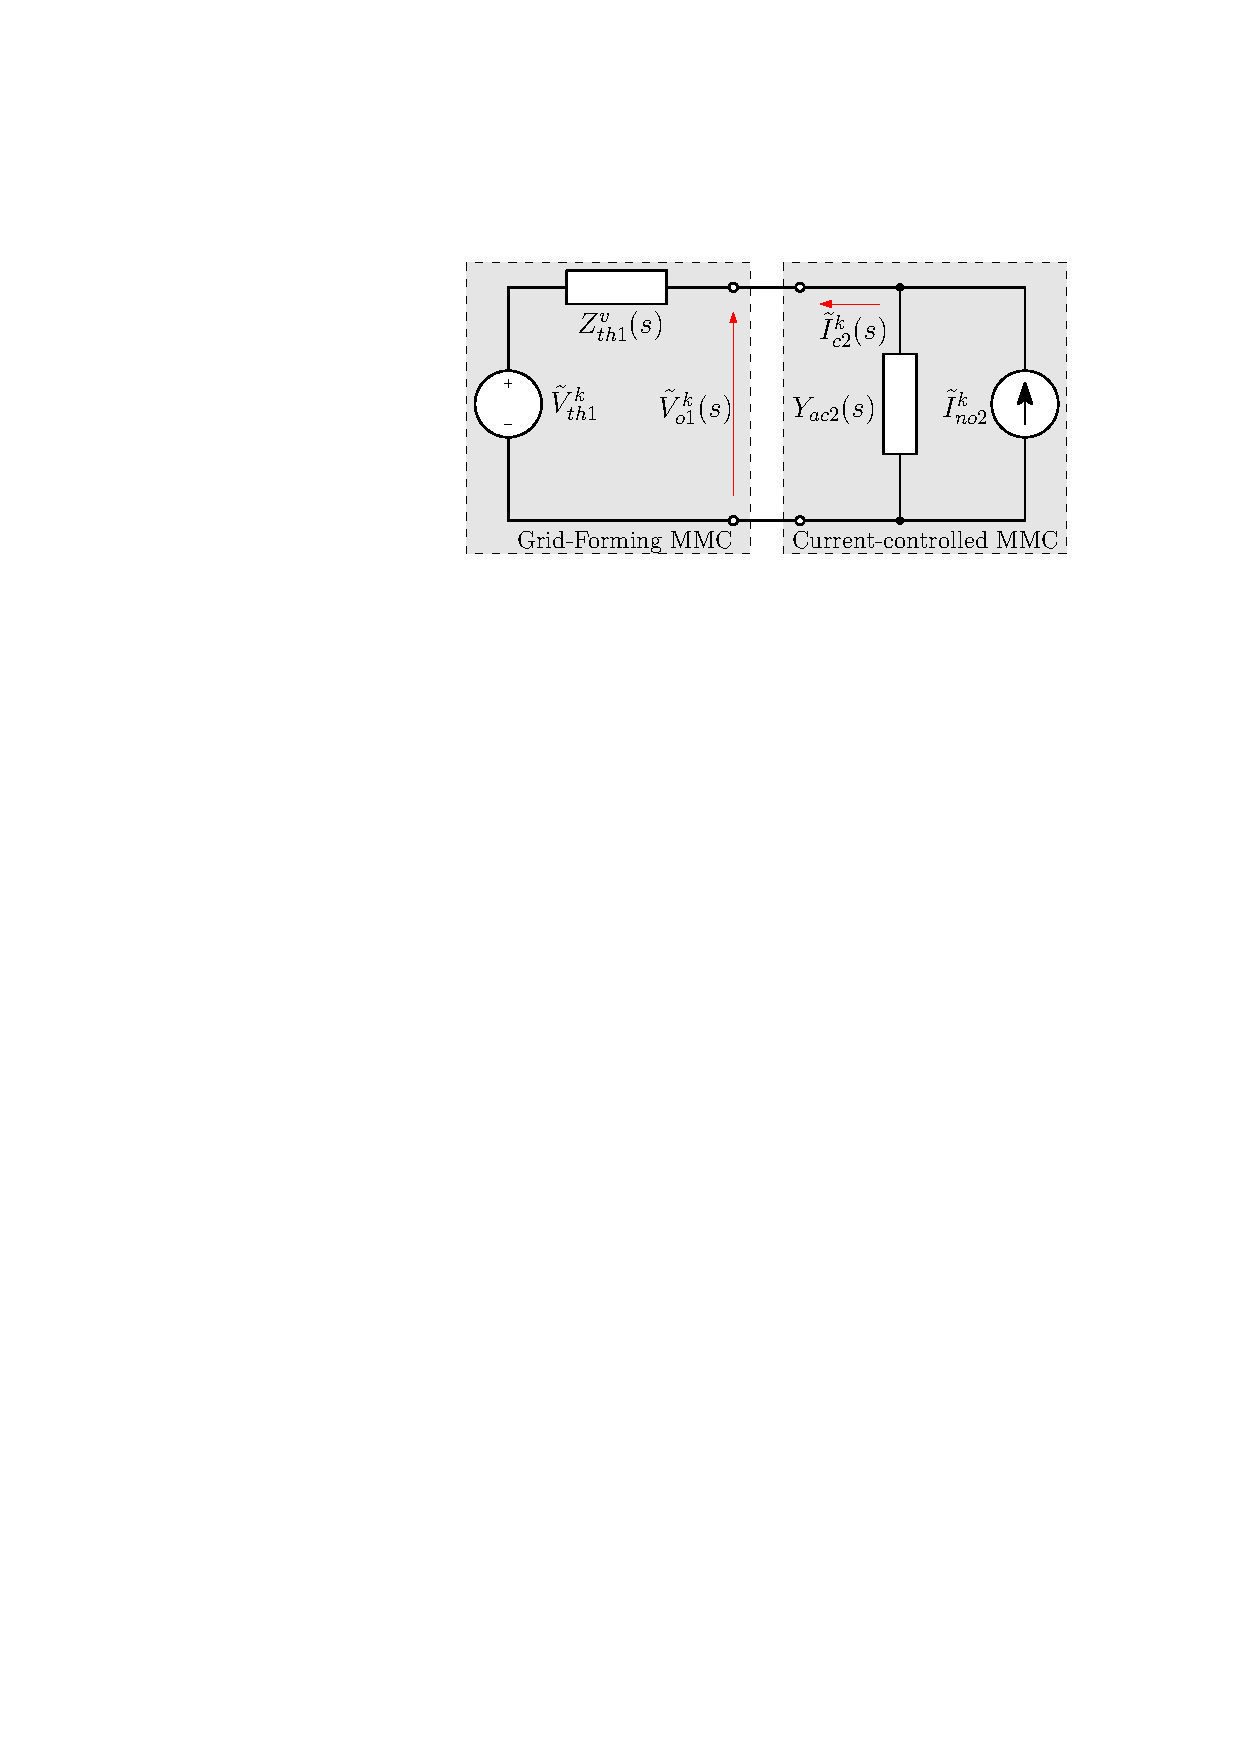
\includegraphics[width=0.85\linewidth]{./figuras/aplicacao/stability_ca}
%
%
%\begin{itemize}
%	\item Um conversor assumindo o papel de fonte de tensão
%	\item Outro assumindo o papel de fonte de corrente
%\end{itemize}
%
%
%\column{0.5\textwidth}
%\centering
%
%\begin{itemize}
%	\item A interação entre os sistemas é dada por:
%	
%	\begin{equation*}
%	\mathcal{L}(s) = Z_{th1}^v(s) Y_{ca2}(s)
%	\end{equation*}\\[10pt]
%
%	\item $\mathcal{L}(s)$ assume o papel de uma função de transferência de malha aberta do sistema\\[10pt]
%	
%	\item Então $\mathcal{L}(s) + 1 = 0$ é a equação característica do sistema  
%\end{itemize}
%
%
%
%
%
%\end{columns}
%
%\end{frame}

%
%%%%%%%%%%%%%%%%%%%%%%%%%%%%%%%%%%%%%%%%%%%%%%%%%%%%%%%
%%%%%%%%%%%%%%%%%%%%%%%%%%%%%%%%%%%%%%%%%%%%%%%%%%%%%%%
%%%%%%%%%%%%%%%%%%%%%%%%%%%%%%%%%%%%%%%%%%%%%%%%%%%%%%%
\begin{frame}{Análise de Estabilidade Baseada em Impedâncias}



\begin{columns}

\column{0.5\textwidth}

Critério definido por Prof. Jian Sun em {\color{blue}\href{https://ieeexplore.ieee.org/document/5741855}{Artigo de 2011}}.\\[20pt] 

\centering
Circuito Equivalente\\[15pt]

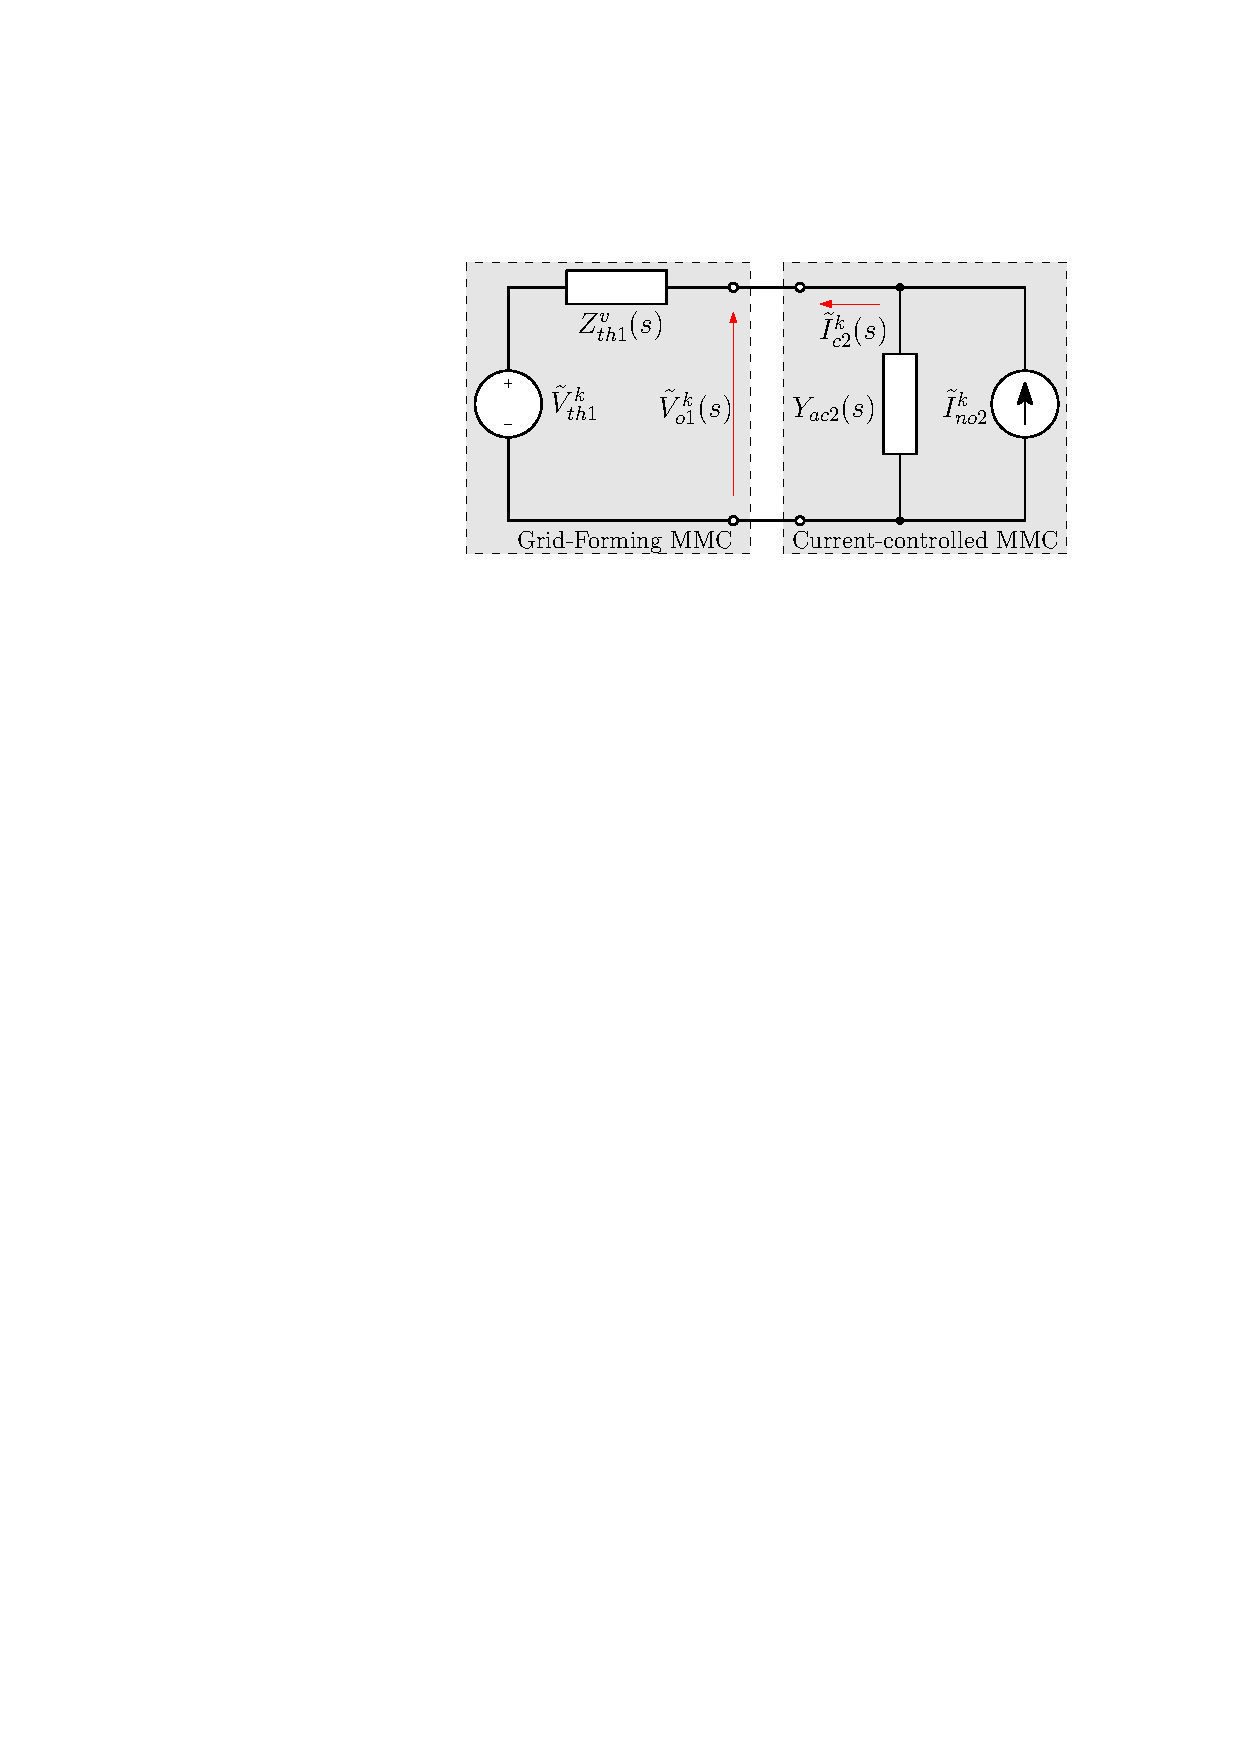
\includegraphics[width=0.85\linewidth]{./figuras/aplicacao/stability_ca}


%\begin{itemize}
%	\item Um conversor assumindo o papel de fonte de tensão
%	\item Outro assumindo o papel de fonte de corrente
%\end{itemize}


\column{0.5\textwidth}
\centering

\begin{itemize}
	\item A interação entre os sistemas é dada por:
	
	\begin{equation*}
	\mathcal{L}(s) = Z_{th1}^v(s) Y_{ca2}(s)
	\end{equation*}\\[10pt]

	\item $\mathcal{L}(s)$ assume o papel de uma função de transferência de malha aberta do sistema\\[10pt]
	
	\item Então $\mathcal{L}(s) + 1 = 0$ é a equação característica do sistema  
\end{itemize}





\end{columns}

\end{frame}

%
%
%%%%%%%%%%%%%%%%%%%%%%%%%%%%%%%%%%%%%%%%%%%%%%%%%%%%%%%%
%%%%%%%%%%%%%%%%%%%%%%%%%%%%%%%%%%%%%%%%%%%%%%%%%%%%%%%%
%%%%%%%%%%%%%%%%%%%%%%%%%%%%%%%%%%%%%%%%%%%%%%%%%%%%%%%%
%\begin{frame}{Resultados}
%
%
%\begin{columns}
%
%\column{0.5\textwidth}
%
%\centering
%{Condição Estável}
%
%
%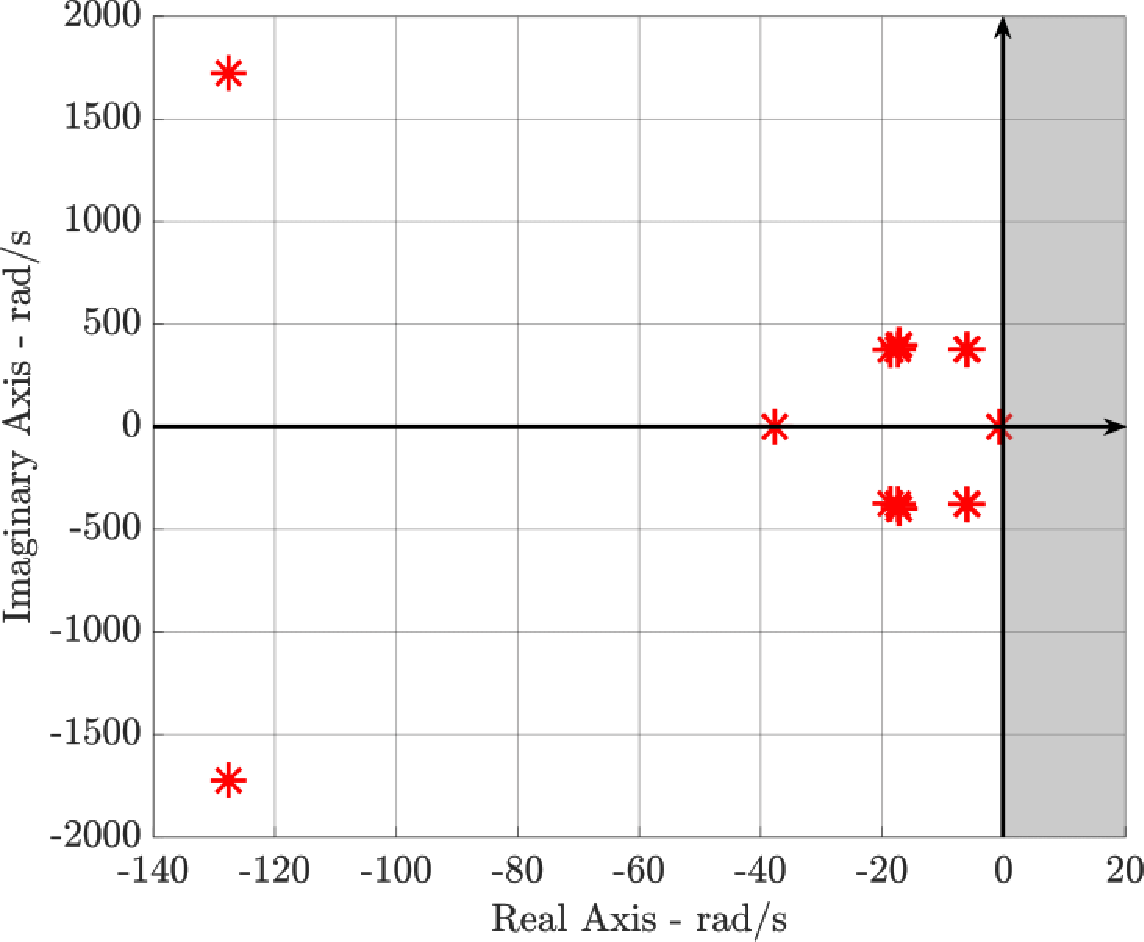
\includegraphics[width=0.45\linewidth]{./figuras/aplicacao/poles_ca_estavel}
%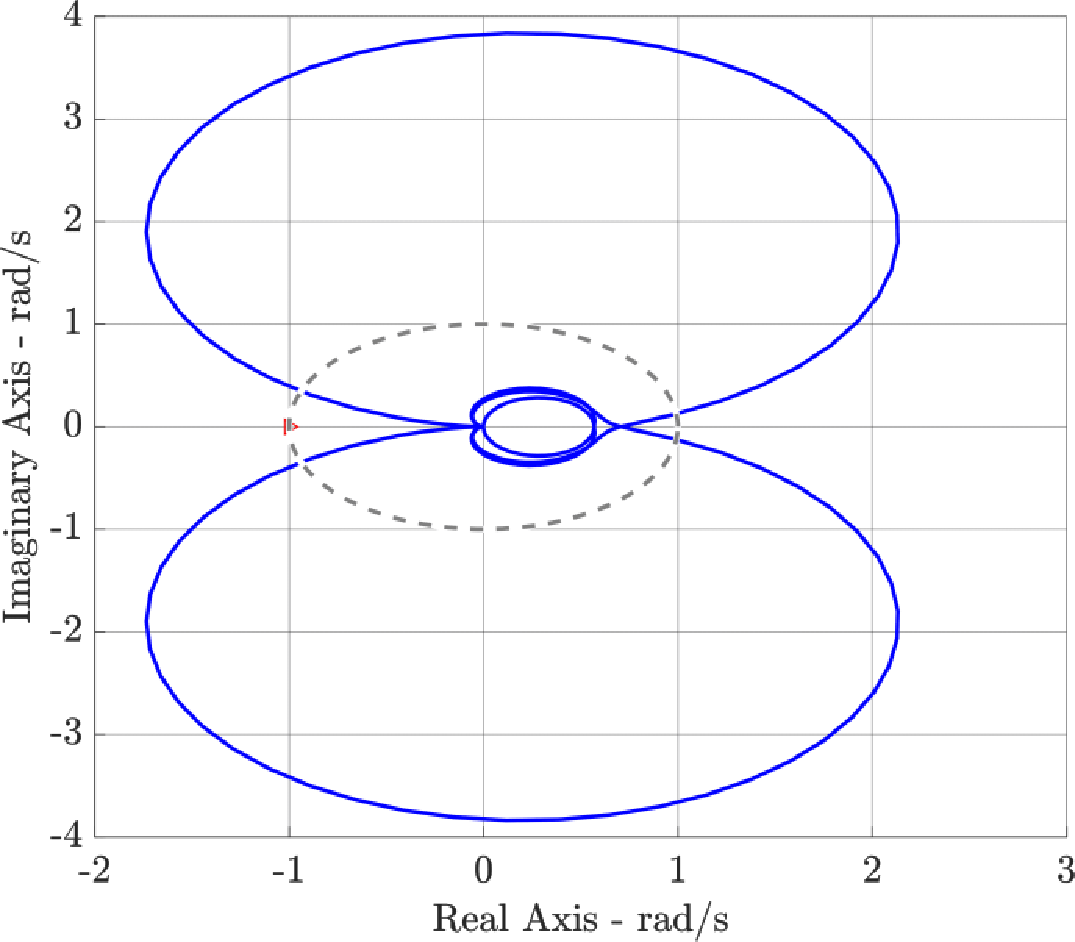
\includegraphics[width=0.42\linewidth]{./figuras/aplicacao/nyquist_ca_estavel}\\
%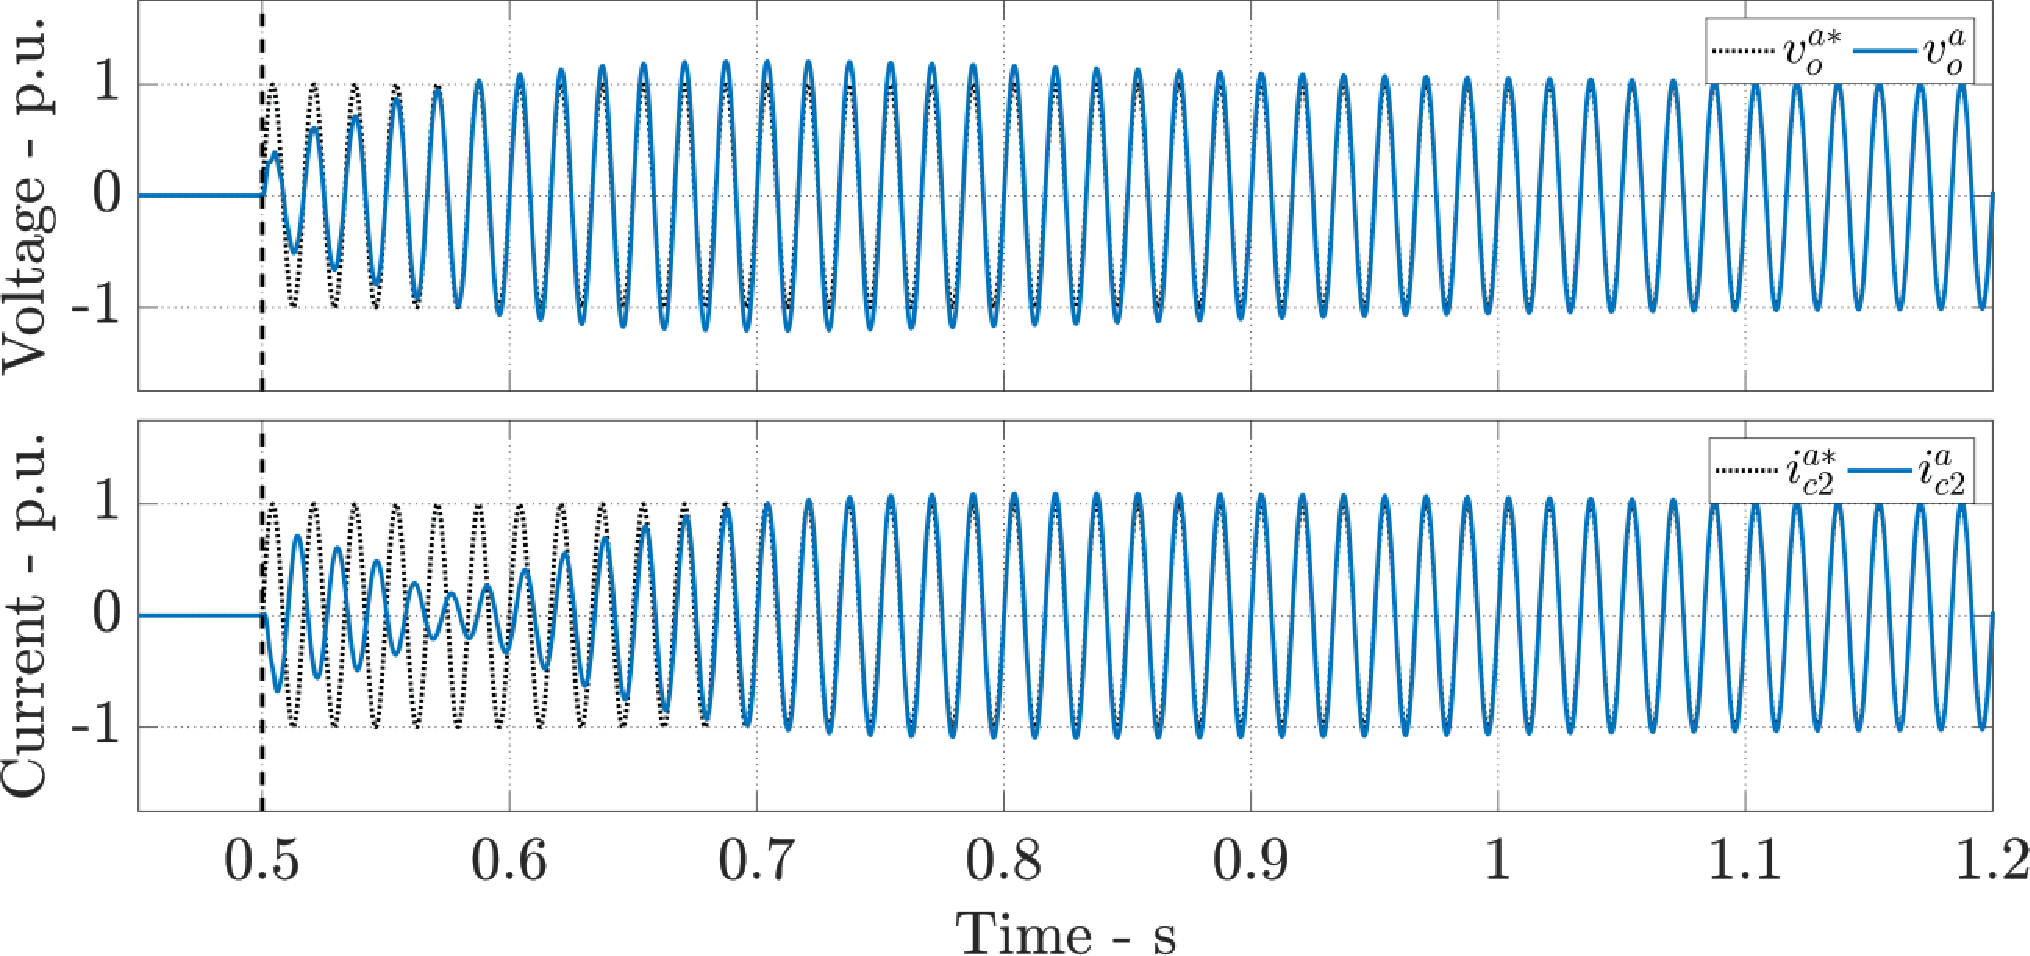
\includegraphics[width=0.95\linewidth]{./figuras/aplicacao/time_resp_ca_estavel}
%
%\column{0.5\textwidth}
%
%\centering
%{Condição Instável}
%
%
%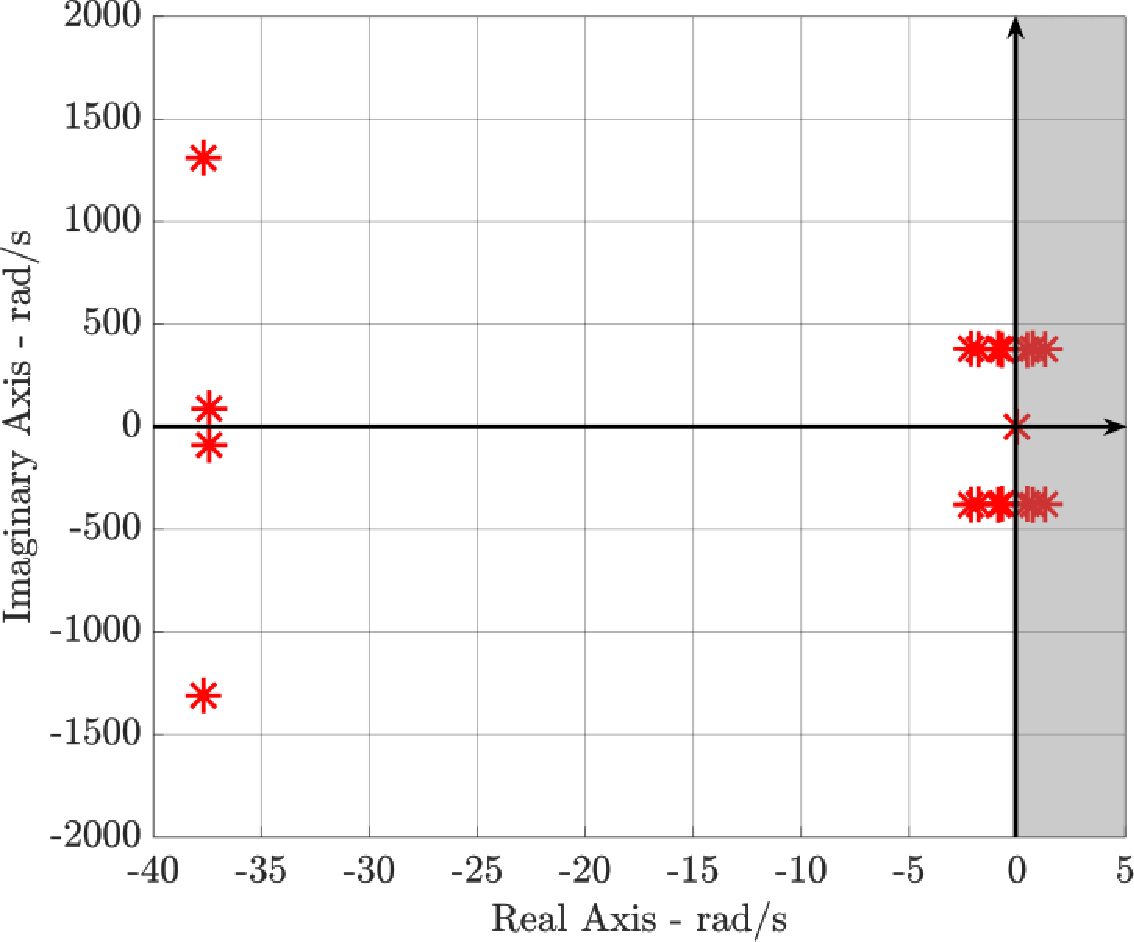
\includegraphics[width=0.45\linewidth]{./figuras/aplicacao/poles_ca_instavel}
%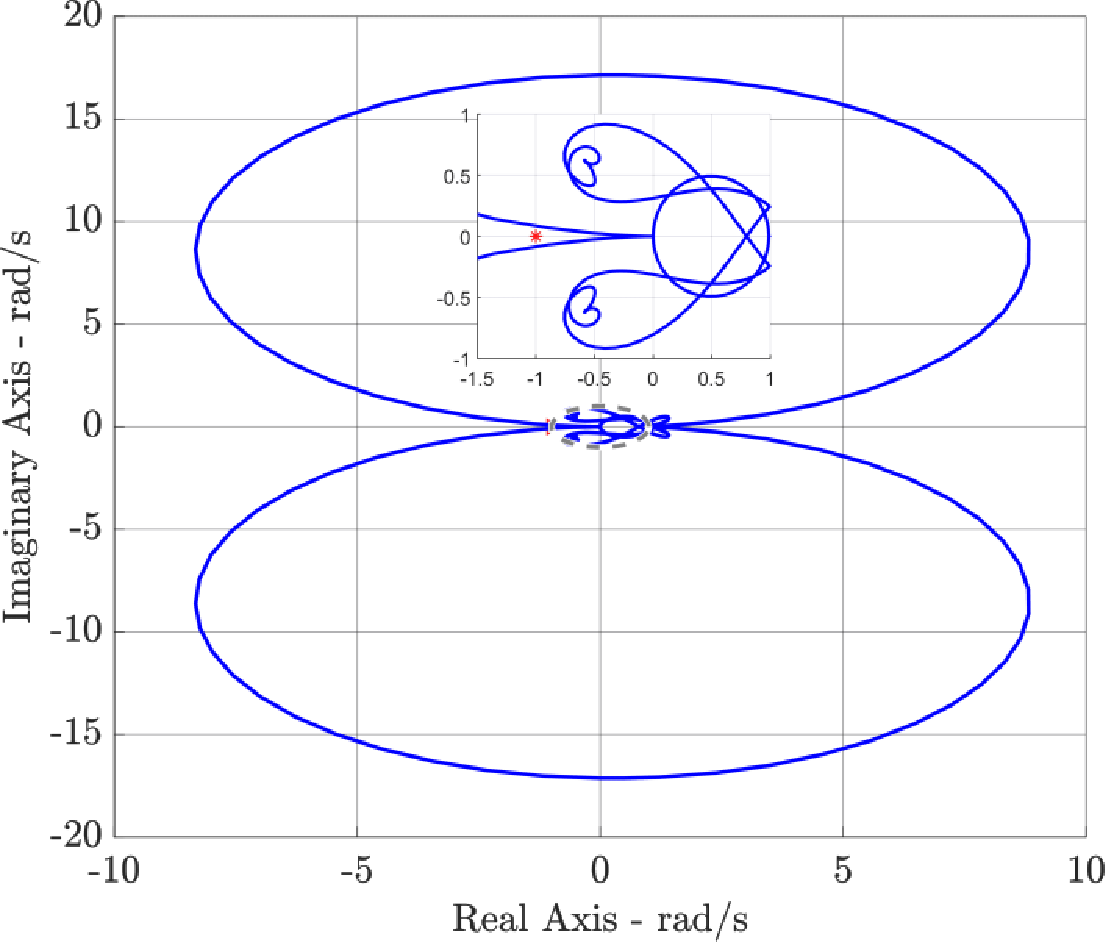
\includegraphics[width=0.42\linewidth]{./figuras/aplicacao/nyquist_ca_instavel}\\
%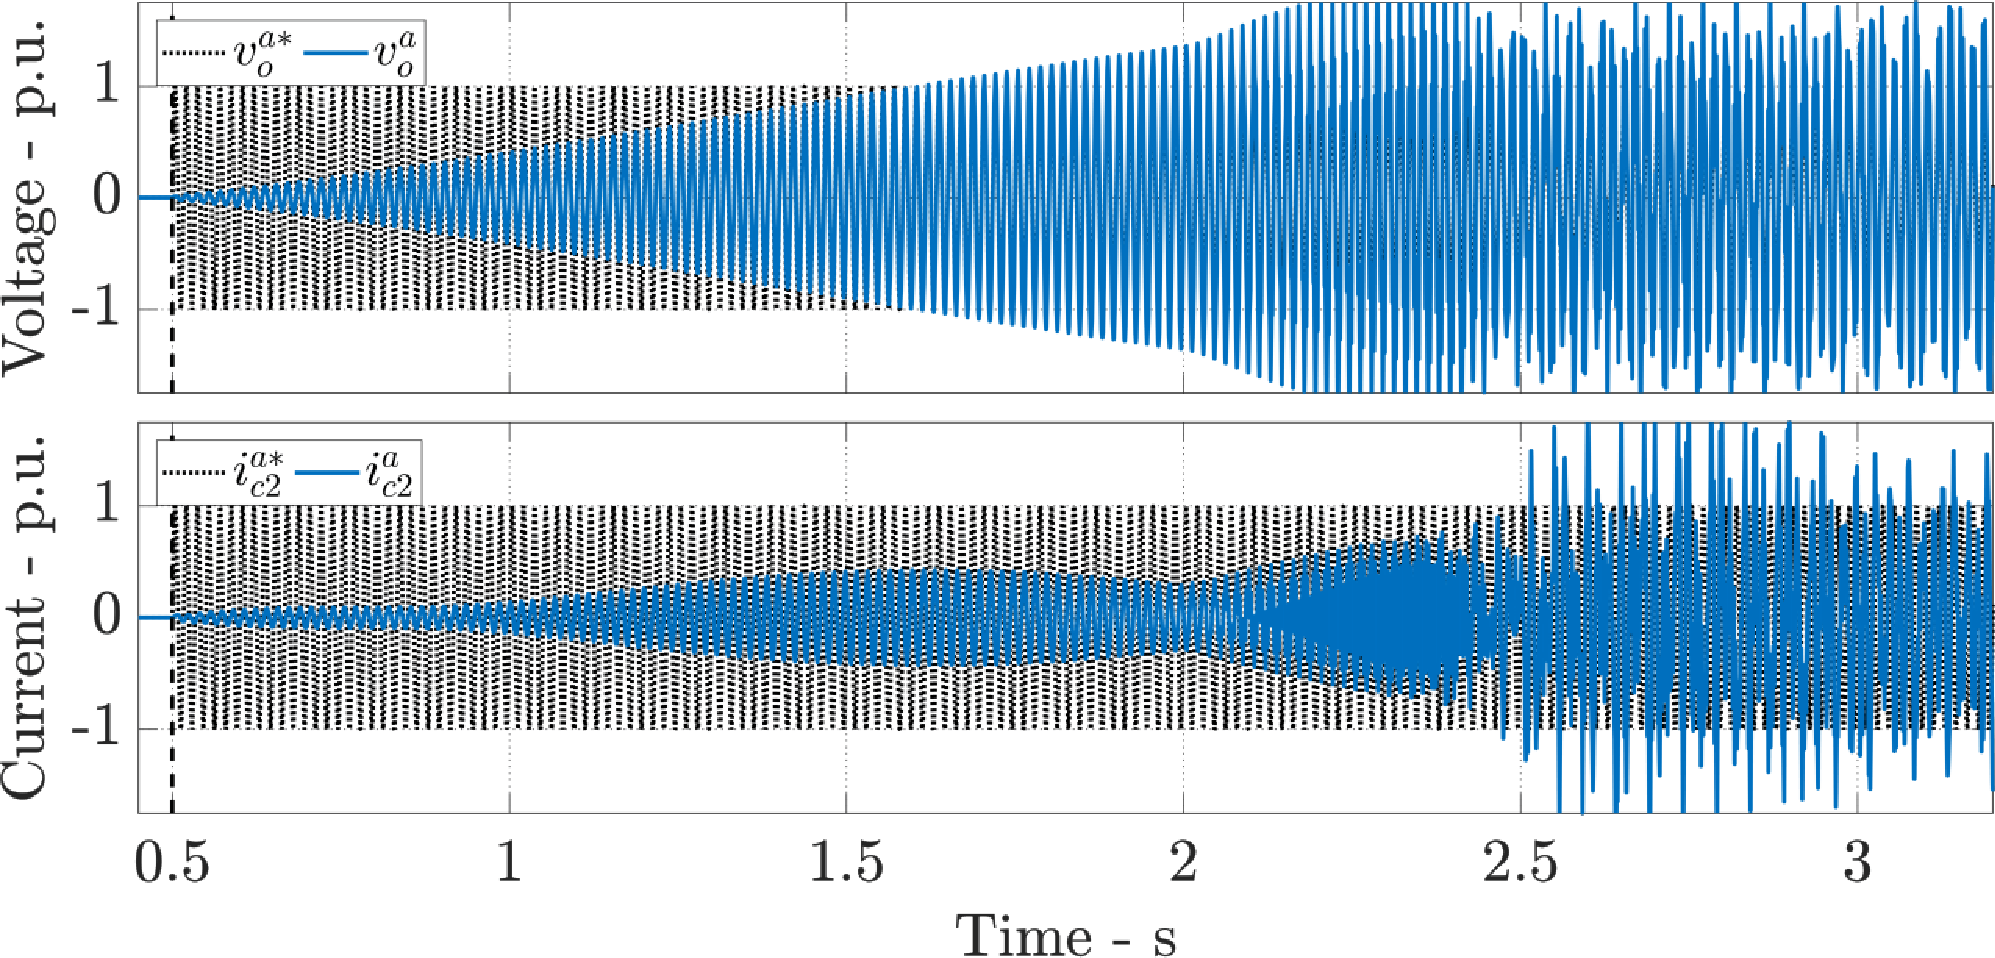
\includegraphics[width=0.95\linewidth]{./figuras/aplicacao/time_resp_ca_instavel}
%
%\end{columns}
%
%\end{frame}
%
%




%%%%%%%%%%%%%%%%%%%%%%%%%%%%%%%%%%%%%%%%%%%%%%%%%%%%%%%
%%%%%%%%%%%%%%%%%%%%%%%%%%%%%%%%%%%%%%%%%%%%%%%%%%%%%%%
%%%%%%%%%%%%%%%%%%%%%%%%%%%%%%%%%%%%%%%%%%%%%%%%%%%%%%%
\begin{frame}{Resultados}


\begin{columns}

\column{0.5\textwidth}
\vspace*{-0.1cm}
\centering
{Condição Estável\\[5pt]}


\begin{columns}
\column{0.5\textwidth}
\centering
\small
Polos de Malha Aberta
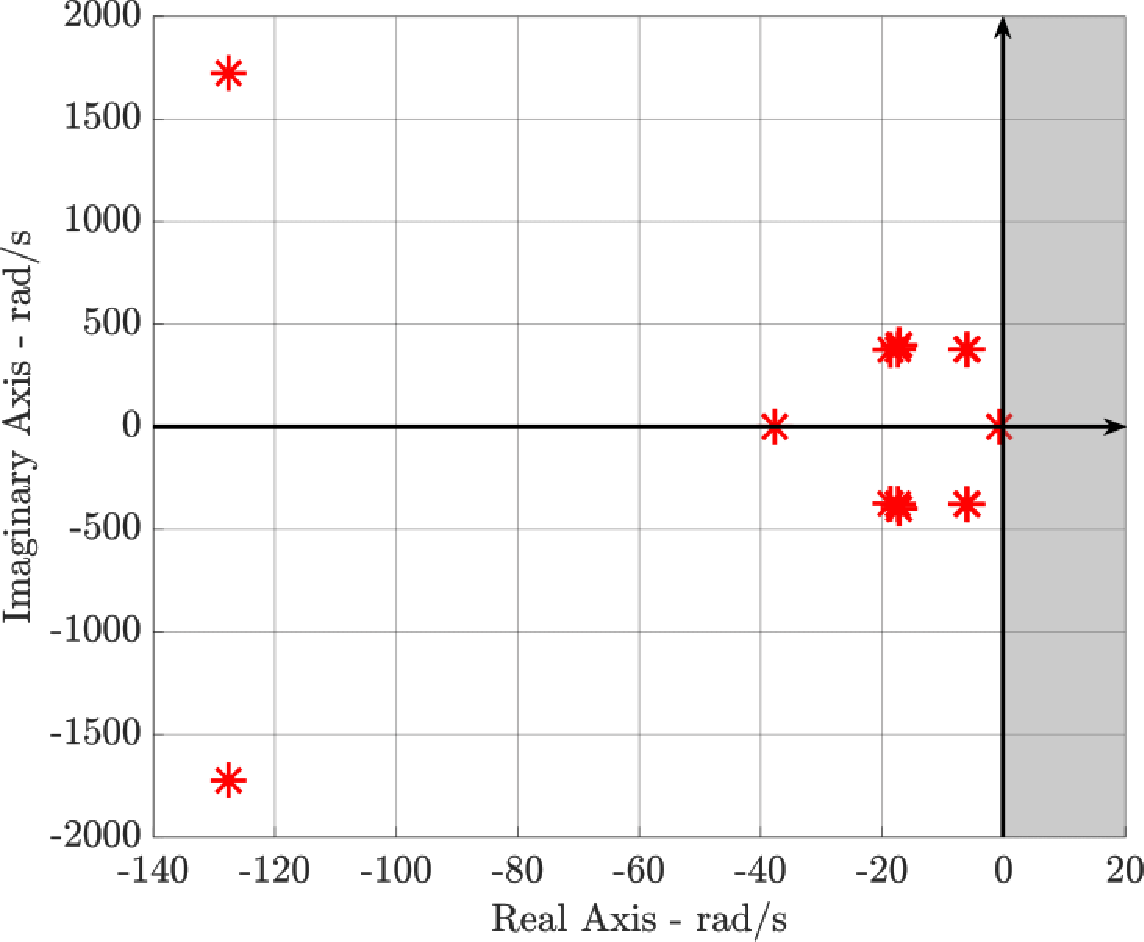
\includegraphics[width=0.80\linewidth, height=2.5cm]{./figuras/aplicacao/poles_ca_estavel}
\column{0.5\textwidth}
\centering
\small
Diagrama de Nyquist
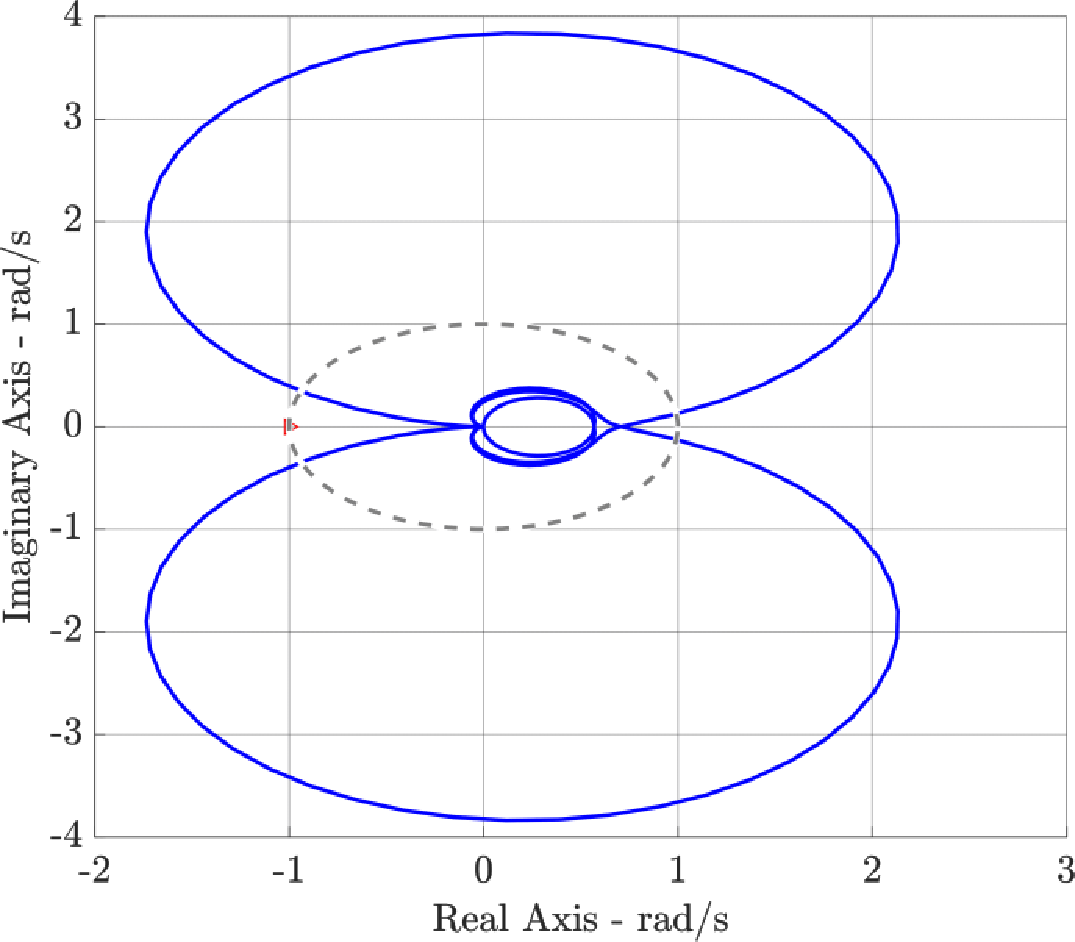
\includegraphics[width=0.75\linewidth, height=2.5cm]{./figuras/aplicacao/nyquist_ca_estavel}
\end{columns}
\small 
Simulação
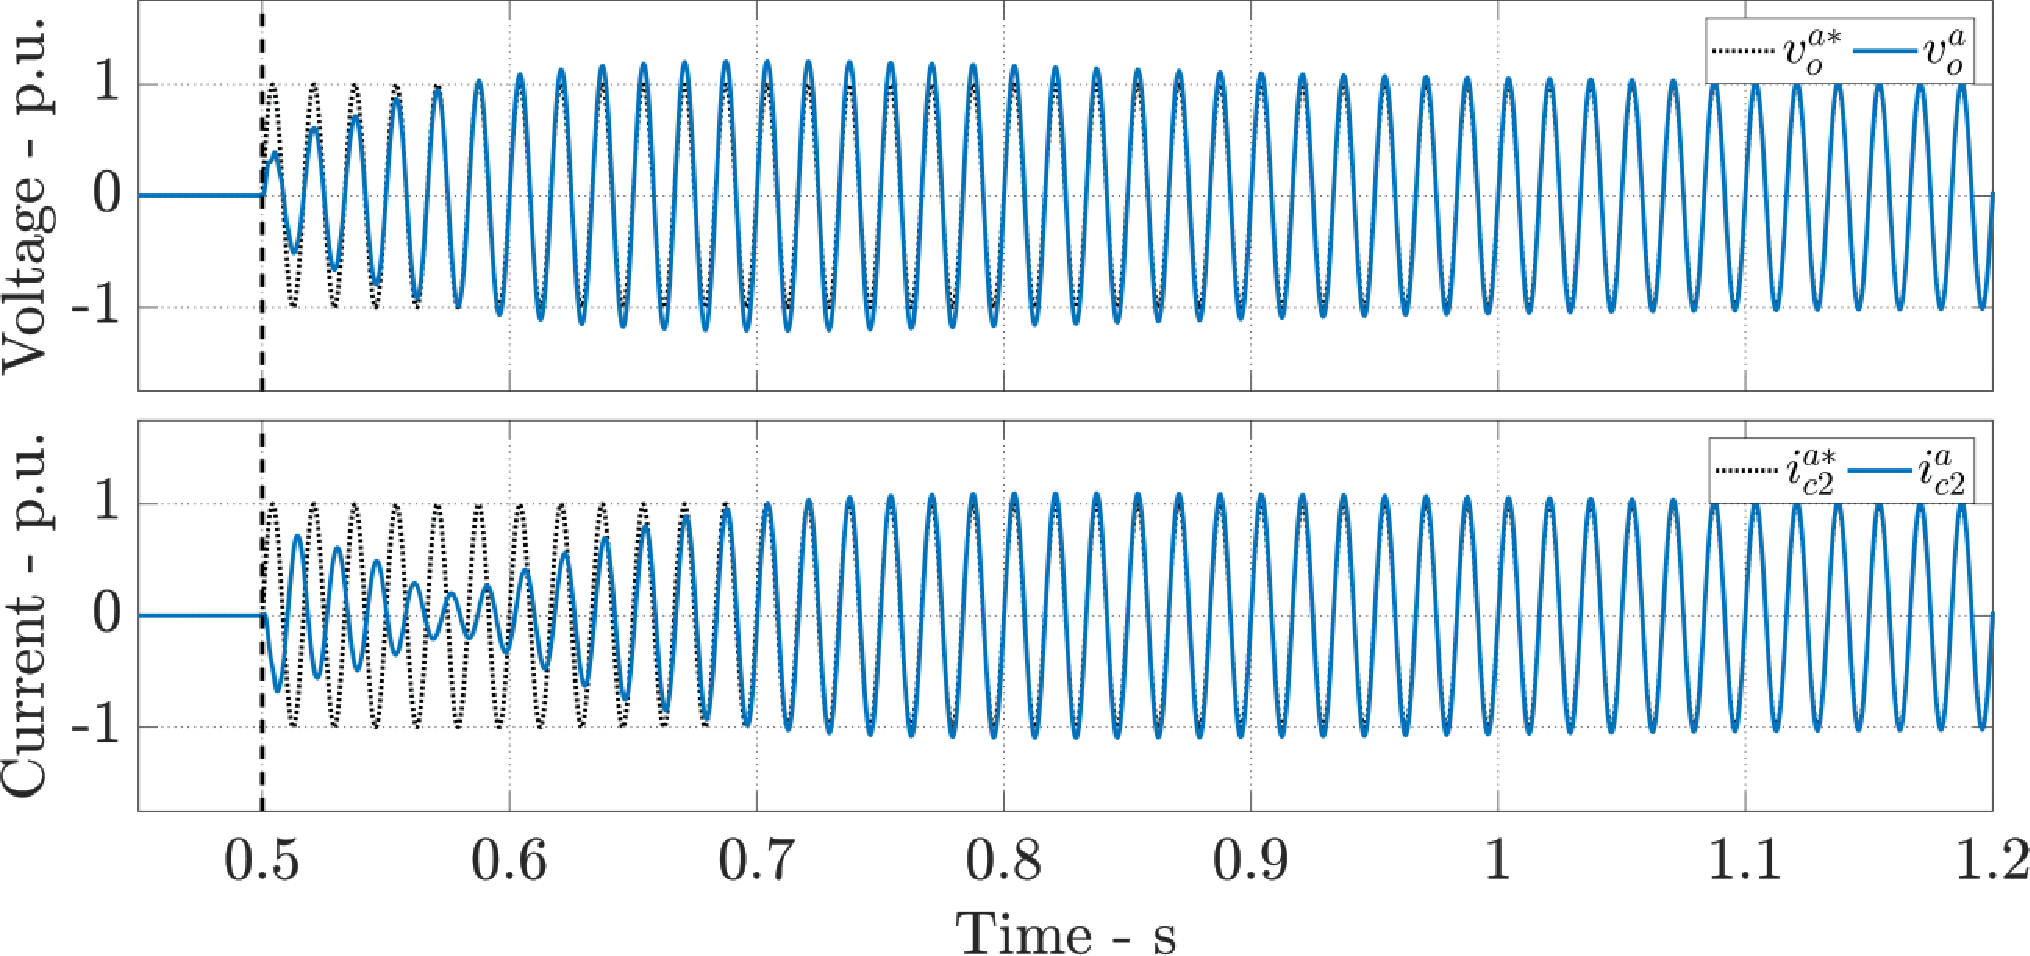
\includegraphics[width=0.96\linewidth]{./figuras/aplicacao/time_resp_ca_estavel}

\column{0.5\textwidth}
\vspace*{-0.1cm}
\centering
{Condição Instável\\[5pt]}


\begin{columns}
\column{0.5\textwidth}
\centering
\small
Polos de Malha Aberta
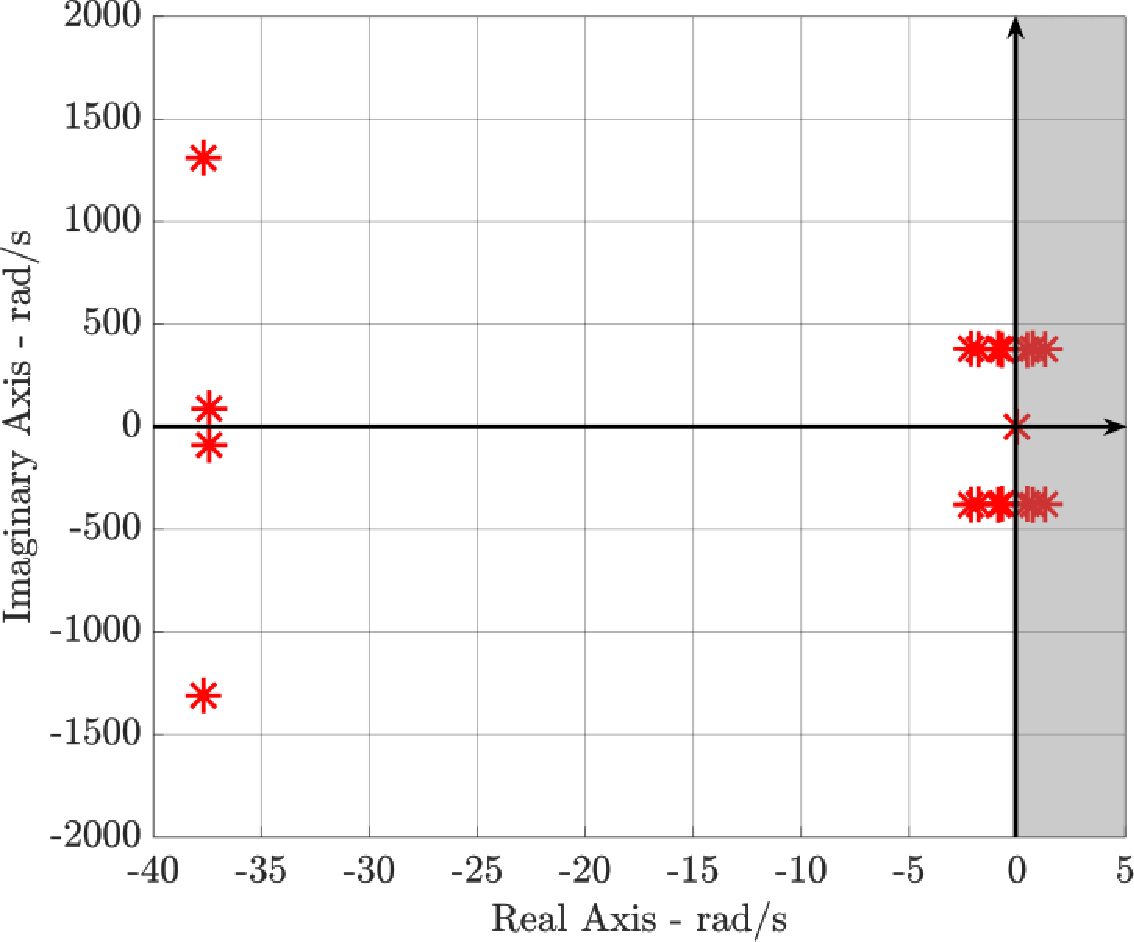
\includegraphics[width=0.80\linewidth, height=2.5cm]{./figuras/aplicacao/poles_ca_instavel}
\column{0.5\textwidth}
\centering
\small
Diagrama de Nyquist
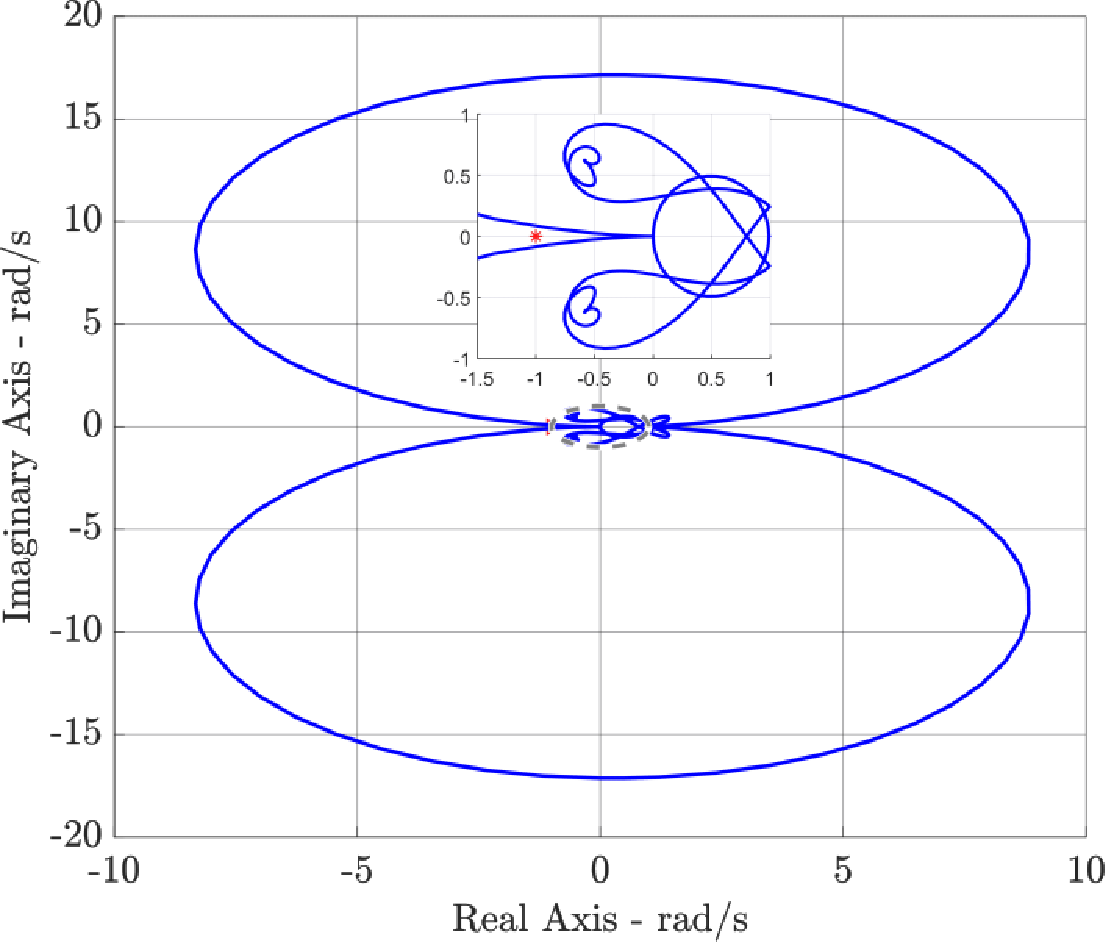
\includegraphics[width=0.75\linewidth, height=2.5cm]{./figuras/aplicacao/nyquist_ca_instavel}
\end{columns}
\small 
Simulação
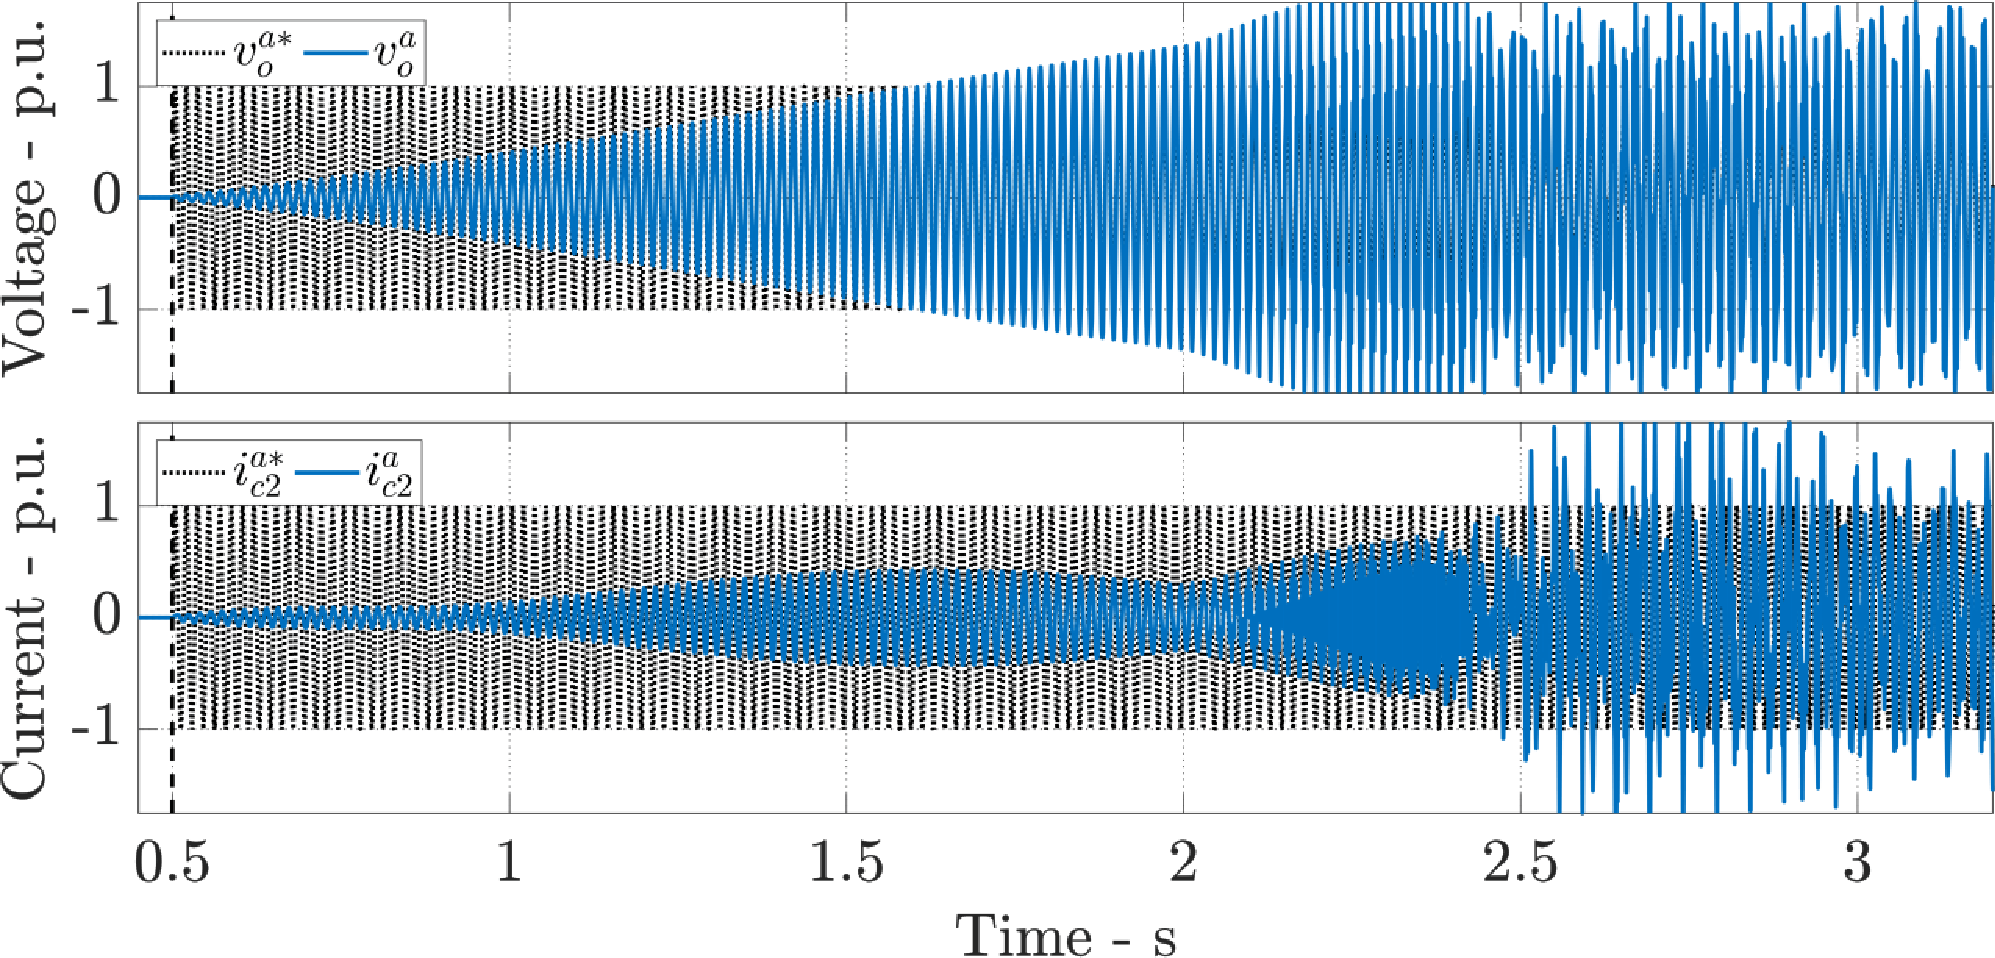
\includegraphics[width=0.96\linewidth]{./figuras/aplicacao/time_resp_ca_instavel}


\end{columns}

\end{frame}



